\subsection{Overview}
\begin{figure}[h!]
	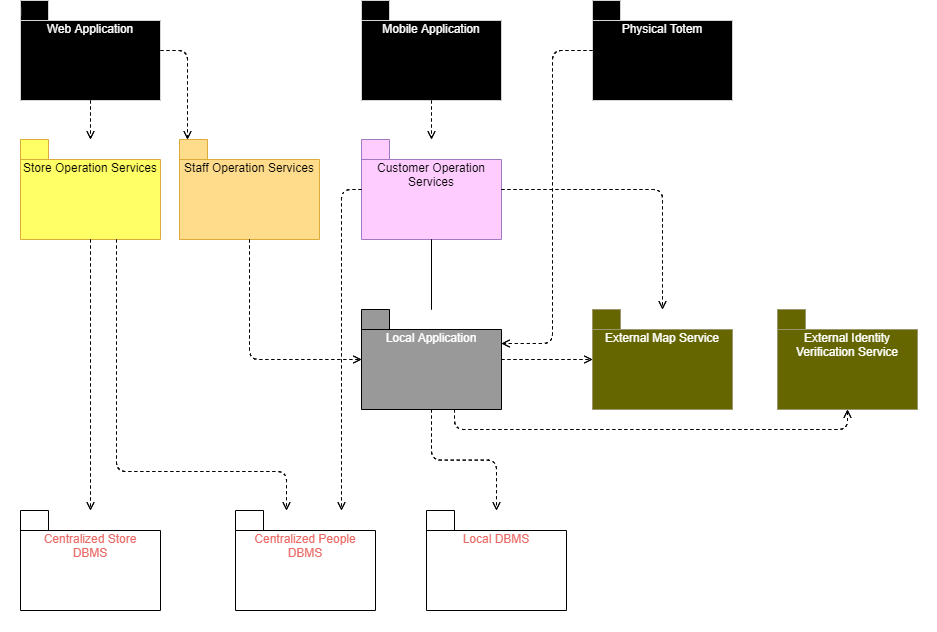
\includegraphics[width=\linewidth]{../Diagrams/IntegrationImplementation/IntegrationOverview.png}
	\caption{Implementation}
	\label{fig:Implementation1}
\end{figure}
In this part there will be an explanation on how and in which order the development, integration and testing of this project should be done. The idea is to complete a end user testable version with the bare minimum functionalities as soon as possible so that then it is possible to test this base extensively while adding the rest of the features.
\subsection{Implementation Plan}
The chosen approach for implementing, testing and integrating the system is bottom-up but by implementing in a first moment just the most basic functionalities of every component.
The aim of this approach is to implement, integrate and test an initial version of the system as soon as possible so that then the missing features can be developed on a functioning base with the minimum need of drivers and stubs and by keeping them simple when they are strictly needed.
This way it is in fact possible to firstly develop completely and properly test the core feature, which is the virtual queuing on the user part, and then add the other features i.e. booking the entrance on a certain time and date (which can partially be seen as an extension of the virtual queuing), ordered stores suggestions given filters and current queues and lastly the store management functions on the store manager’s part.
Thus the development of each component will be incremental once an initial version of the system with basic features from start to end is finished.
\\

The development has to start with configuring the \textbf{Local DBMS} and creating the \textbf{Local Application} component (an instance of it will be hosted by every registered store), this component is in fact is the core of the management of information about queues, bookings, user reports and user notifications, and practically feeds the CLup system and clients with operational information. For now only the queues and notifications subcomponents will be developed. Also the interface with the physical totems (part of the queuing process) will be developed in order to allow people to queue in the stores even if they don’t use the client application, which is part of the basic functionality. At this stage the \textbf{external components} will be connected to the system, they will not require any testing on their own since they come from sources that are assumed trustable and reliable.

After this the development of three more components can start: on the store side \textbf{Staff Operation Services}, which is needed for the functioning of the web app’s control panel available to the store managers, for now only its functionality to allow and stop store entrances which is part of the \textit{StoreAvailabilityManagement} subcoponent will be developed; on CLup’s server side the components \textbf{Store Operation Services} together with \textbf{Centralized Store and People DBMSs} and \textbf{Customer Operation Services} can be developed/configured, the former with just the \textit{StoreManagement} subcomponent while the latter with only the \textit{StoreAvailabilityManagement}, according to what was developed in Local Application (e.g. no booking management).\\

Now it is possible to develop the user interfaces for each module: the \textbf{Mobile Application} for the smartphone users, the \textbf{Web Application} for the store managers and the \textbf{Physical Totem} software for those who don’t use the application. For each of these interfaces (for now) it’s enough to implement interactions just for those functions of the system that have already been developed.\\

After these steps there should be a functioning system composed of a mobile application, a program to be installed on store servers, a program to be deployed on physical totems and a system to be used on the main CLup servers to allow interactions between the previous: with these you should be able to accomplish the basic tasks objective of the purpose of this project such as register users, stores, do logins, get tickets to virtually queue in stores and enter and exit them with such tickets (it has to be noted that for the actually complete testing of the system there needs to be turnstiles and also proper machines for the totems in order to print tickets deployed at the store). The testing can then proceed on this basic version of CLup while the development keeps going on by implementing the missing features described in the RASD: the possibility for users to book entrances, algorithms to properly sort and suggest stores and times to go shopping and the other functions for the store manager’s web app.
Components wise the order in which to implement the various parts of these features over the existing parts of the system is the same as the one previously described.
Summing up the implementation order goes in 3 phases with respective components: \begin{enumerate}
	\item The stores’ local application: Local DBMS and Local Application
	\item Central CLup system and local store interaction with this system: Staff Operation Services, Store Operation Services, Customer Operation Services, Centralized People and Centralized Store DBMSs
	\item The users and store staff interfaces: Web Application, Mobile Application and Physical Totem
\end{enumerate}




\subsection{Integration Strategy}
The integration of the components follows their implementation, so that no components will remain isolated at any time during development in order to avoid the risk of inconsistencies between them.
\begin{enumerate}
	\item In a first moment the \textbf{Local DBMS} and \textbf{Local Application} are integrated, also the two \textbf{external components} are integrated in the system. A \textbf{stub} and a \textbf{driver} are used to simulate the components supposed to interact with the local application, anyway they don’t need to be complex at all since all that is being implemented and integrated for now is just the basic functionalities and subcomponents, so Bookings and Reports will be left out for now.
	\begin{figure}[H]
		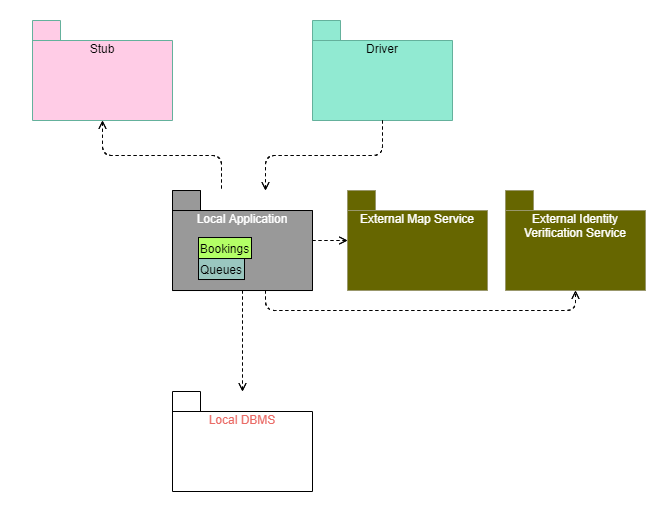
\includegraphics[width=\linewidth]{../Diagrams/IntegrationImplementation/Integration1st.png}
		\caption{First step of the integration}
		\label{fig:Implementation2}
	\end{figure}
	\item Then \textbf{Staff Operation Services} is integrated with local application, also \textbf{Store} \textbf{Operation Services} with its \textbf{DBMSs} joins the system since they both share a \textbf{driver} for the Web Application. The other part of the central CLup’s system can also be integrated since Local Application is ready: \textbf{Customer Operation Services}, there will be a \textbf{driver} for this part representing the mobile app and also a \textbf{driver} for the totem will remain from the previous step.
	\begin{figure}[H]
		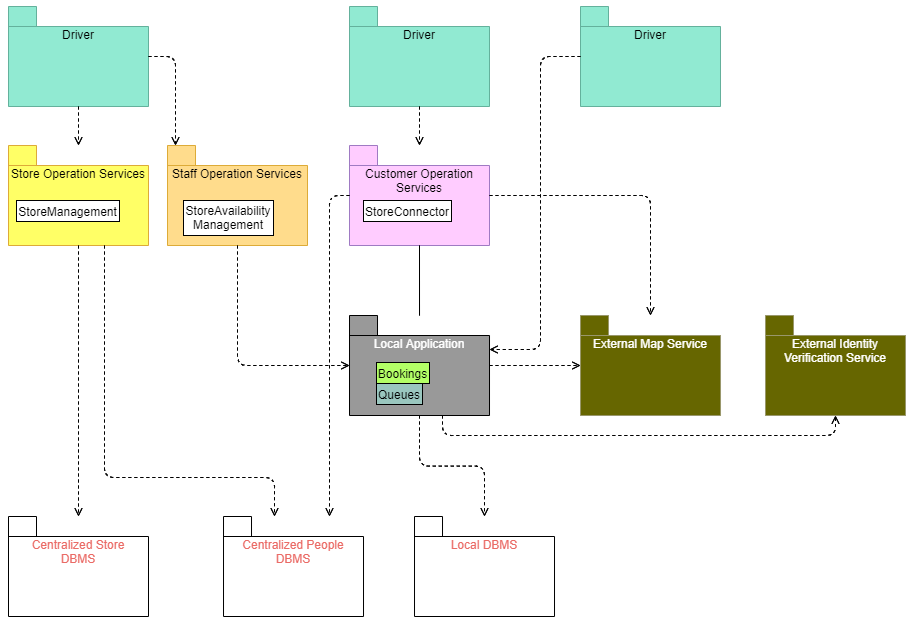
\includegraphics[width=\linewidth]{../Diagrams/IntegrationImplementation/Integration2nd.png}
		\caption{Second step of the integration}
		\label{fig:Implementation3}
	\end{figure}
	\item Lastly the user \textbf{interfaces} are integrated in order to complete the initial version of the project.
	\begin{figure}[H]
		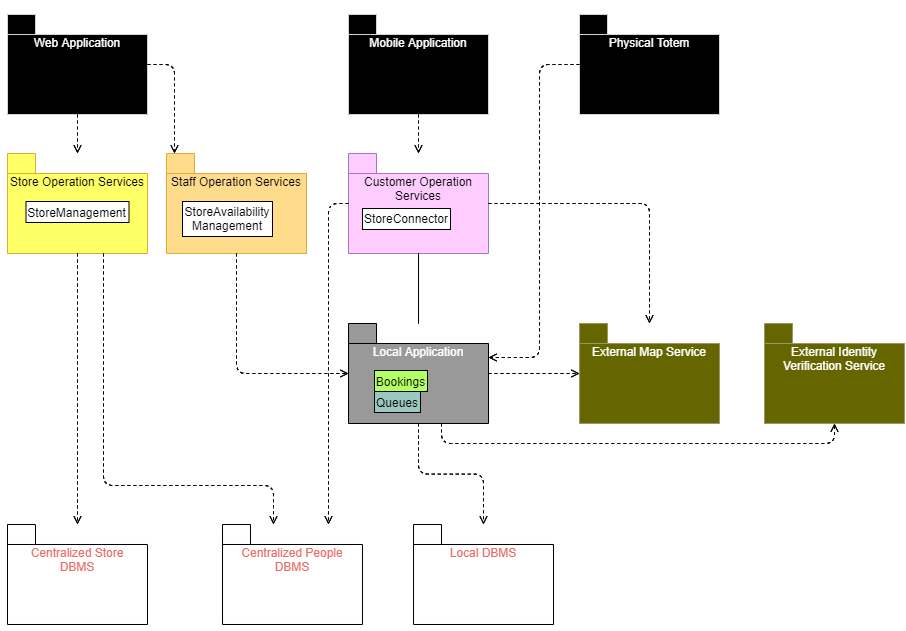
\includegraphics[width=\linewidth]{../Diagrams/IntegrationImplementation/Integration3rd.png}
		\caption{Third step of the integration showing the first version of the system capable of offering the basic functionalities}
		\label{fig:Implementation4}
	\end{figure}
	\item Now the remaining sub components will integrated following the order in which their respective components were integrated explained in this section.
	\begin{figure}[H]
		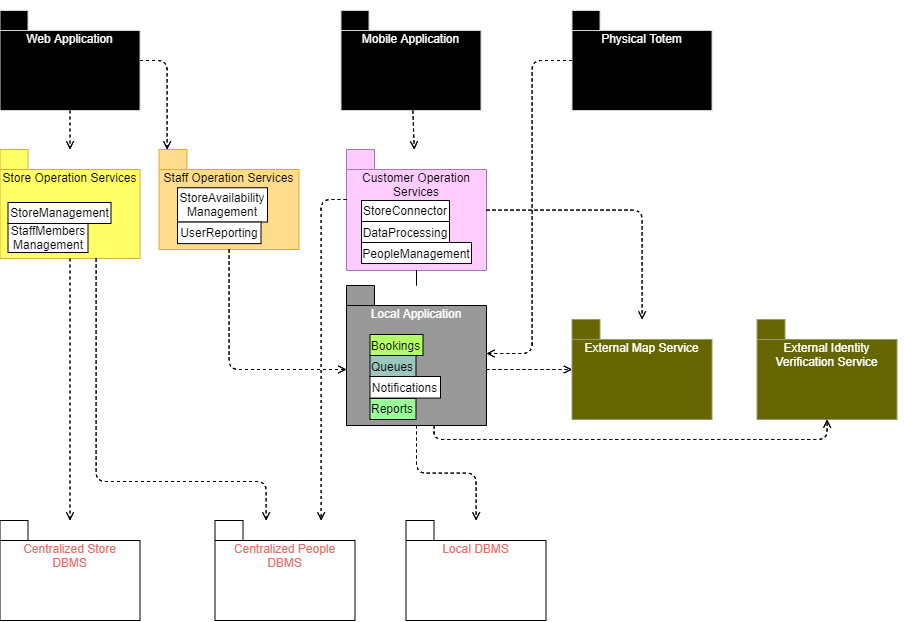
\includegraphics[width=\linewidth]{../Diagrams/IntegrationImplementation/IntegrationFull.png}
		\caption{End of the integration showing the complete system}
		\label{fig:Implementation5}
	\end{figure}
\end{enumerate}

\subsection{System Testing}
Upon the completion of the basic version of the system, again at the completion of each system feature, and most importantly after the implementation and integration of every feature, the system must be tested in its entirety. The tests are meant to verify the satisfaction of both functional and nonfunctional requirements.\\

Common practices guide us on the types of tests we have to perform:
\begin{enumerate}
	\item Functional testing: verify the satisfaction of the RASD functional requirements
	\item Performance testing: find bottlenecks, response times affected, utilization and throughput, also run benchmarks
	\item Load testing: identify upper limits for workload and expose possible bugs in memory management and buffer overflows
	\item Stress testing: reveal how the system recovers from failures such as unexpected shutdowns and disconnections
\end{enumerate}

\subsection{Additional Specification on Testing}
Here we will present some guidelines on how to analyse, test, verify and validate the project.

First of all an initial analysis over the RASD and DD documents should be conducted by a quality team.
The analysis is divided in walkthrough and inspection, the first one should be performed in meetings with experts on the field of this project in order to do an initial check of its correctness for its purpose.
The second one also has to be performed, it focuses more on the formal aspects and is done by professional inspectors who will follow a checklist of things to be examined.
The inspection activity must continue during the entire development since it will also check the generated code and it will also consist in meetings where the members of the developer team have to partecipate.
The job of the quality team is to just report problems in the code while the developers have to be the ones correcting such problems, the fixes then will be checked again by the quality team.
It is very important that the code is properly commented in a semi-formal way by the developers, so that the quality team can expect standardized work to analyse.
Apart from the inspection work, in order to find problems with the code, effort must also be done by the developers in the generation of test cases which should cover at least 90\% of the code, since this will help find problems earlier than the inspection.
As previously mentioned the aim is to have an usable application with basic functionalities as soon as possible, so when it will be ready an additional team of testers will go through it and its next versions to test and evaluate the integrated system.
The code testing has to be white-box systematic since this is incentivated by the bottom up approach and almost all the components are going to be built from scratch.

